\chapter{Systems of ODEs}

\section{First-order systems of ODEs}
Consider the following:
\begin{equation*}
\ddot{x} + x \dot{x} + \sin x = 0
\end{equation*}

This is a 2nd order, non-linear ODE. We can think of this as a system of ODEs by letting $y = \dot{x}$, so $\dot{y} = \ddot{x}$. Then we can rewrite the above as:
\begin{equation*}
\begin{cases}
\dot{x} = y \\
\dot{y} = -x y - \sin x
\end{cases}
\end{equation*}

While this is a first-order system of ODEs, the solution is now two-dimensional, so we can represent it as a vector:
\begin{equation*}
\begin{bmatrix}
\dot{x} \\
\dot{y}
\end{bmatrix} =
\begin{bmatrix}y \\
-x y - \sin x
\end{bmatrix}
\end{equation*}

We call this a \textbf{phase space} representation of the system. The solution to this system will be a curve in the $xy$-plane, which we can visualize as a trajectory of the system.

\dfn{Linear system of ODEs}{
    A system of ODEs is linear if it can be written in the form:
\begin{equation*}
\dot{u} = 
\begin{bmatrix}
\dot{x}_1 \\
\dot{x}_2 \\
\vdots \\
\dot{x}_n
\end{bmatrix} =
\begin{bmatrix}
a_{11} & a_{12} & \cdots & a_{1n} \\
a_{21} & a_{22} & \cdots & a_{2n} \\
\vdots & \vdots & \ddots & \vdots \\
a_{n1} & a_{n2} & \cdots & a_{nn}
\end{bmatrix}
\begin{bmatrix}x_1 \\
x_2 \\
\vdots \\
x_n
\end{bmatrix}
\end{equation*}
}

Letting the matrix be $A$, we can write a linear system of ODEs as:
\[
\boxed{
\dot{u} = A u
}
\]

\nt{
    If $A$ was a 1x1 matrix, then this would be a scalar and hence a single ode of the form:
\begin{equation*}
\dot{u} = \lambda u
\end{equation*}
which we solve as:
\begin{equation*}
u(t) = u(0) e^{\lambda t}
\end{equation*}
}

Now, let $A \in \bbR^{m \times n}$, and let $u(t) \in \bbR^n$ be a vector of functions. Then we can write the system of ODEs as:
\begin{equation*}
\dot{u}(t) = A u(t)
\end{equation*}

We guess that the solution is of the form:
\begin{equation*}
u(t) = e^{At} u(0)
\end{equation*}

However, we must define what $e^{At}$ means.

Recall the Taylor series expansion of the exponential function:
\begin{equation*}
e^{\lambda t} = \sum_{k=0}^{\infty} \frac{(\lambda t)^k}{k!}
\end{equation*}

Then we can define the matrix exponential as:
\begin{equation*}
e^{At} = \sum_{k=0}^{\infty} \frac{(At)^k}{k!}
\end{equation*}

We take the first derivative of $e^{At}$:
\begin{equation*}
\frac{d}{dt} e^{At} = \sum_{k=0}^{\infty} \frac{A^k t^{k-1}}{(k-1)!} = A \sum_{k=0}^{\infty} \frac{(At)^k}{k!} = A e^{At}
\end{equation*}

Thus, we have:
\begin{equation*}
u(t) = e^{At} u(0)
\end{equation*}
is indeed a solution to the system of ODEs.

In particular, we found that $\dot{u}(t) = A e^{At} u(0) = A u(t)$, which is exactly the system of ODEs we wanted to solve.

\ex{Trivial example}{
    Let $\dot{u} = Au$ where:
\begin{equation*}
A = \begin{bmatrix}
    a & 0 \\
    0 & d
\end{bmatrix}
\end{equation*}

Then we let:
\begin{equation*}
\begin{bmatrix}
\dot{x} \\
\dot{y}
\end{bmatrix} =
\begin{bmatrix}
    a & 0 \\
    0 & d
\end{bmatrix}
\begin{bmatrix}
x \\
y
\end{bmatrix} =
\begin{bmatrix}
    a x \\
    d y
\end{bmatrix}
\end{equation*}

Then solving each equation separately, we get:
\begin{equation*}
x(t) = x(0) e^{a t}, \quad y(t) = y(0) e^{d t}
\end{equation*}

\begin{equation*}
\Rightarrow u(t) = \begin{bmatrix}
x(0) e^{a t} \\
y(0) e^{d t}
\end{bmatrix} = e^{At} u(0)
\end{equation*}

where 
\begin{equation*}
u(0) = \begin{bmatrix}
x(0) \\
y(0)
\end{bmatrix}
\end{equation*}
}

Consider each of the cases:
\begin{itemize}
\item $a = d < 0$: then the solution decays to zero as $t \to \infty$. Stability is achieved in both cases.
\item $a = d > 0$: then the solution grows exponentially as $t \to \infty$. Stability is never achieved.
\item $a < d < 0$: then the solution decays to zero as $t \to \infty$, but the $y$ component decays faster than the $x$ component. Stability is achieved in both cases.
\item $d < a < 0$: then the solution decays to zero as $t \to \infty$, but the $x$ component decays faster than the $y$ component. Stability is achieved in both cases.
\item $a < 0 < d$: then the solution decays to zero as $t \to \infty$, but the $x$ component decays while the $y$ component grows. Stability is never achieved.
\item $d < 0 < a$: then the solution decays to zero as $t \to \infty$, but the $y$ component decays while the $x$ component grows. Stability is never achieved.
\end{itemize}

\section{General solution to linear systems of ODEs}
Let $\dot{u} = Au$ where $u = \begin{bmatrix}x_1 \\
x_2 \\
\vdots \\
x_n
\end{bmatrix}$ and $A \in \bbR^{n \times n}$.

We will use the eigenvalue decomposition of $A$ to find the general solution to this system of ODEs. Let $A = PDP^{-1}$ where $D$ is a diagonal matrix containing the eigenvalues of $A$, and $P$ is a matrix whose columns are the corresponding eigenvectors.

Recall the eigenvector $v$ corresponding to an eigenvalue $\lambda$ satisfies:
\begin{equation*}
Av = \lambda v
\end{equation*}

Then we have:
\begin{equation*}
(A - \lambda I) v = 0
\end{equation*}

We find that this is equivalent to stating that $\det(A - \lambda I) = 0$ (remember that the determinant is zero if and only if the matrix is singular, which is the case when there is a non-trivial solution to the above equation). 

Then, solving:
\begin{align*}
\det(A - \lambda I) &=
\begin{vmatrix}
a_{11} - \lambda & a_{12} & \cdots & a_{1n} \\
a_{21} & a_{22} - \lambda & \cdots & a_{2n} \\
\vdots & \vdots & \ddots & \vdots \\
a_{n1} & a_{n2} & \cdots & a_{nn} - \lambda
\end{vmatrix} \\
&= 0 \\
&= \prod_{i=1}^n (\lambda_i - \lambda) = 0
\end{align*}

For a two-dimensional system, we see that the trace and determinant appear in the characteristic polynomial:
\begin{align*}
\det(A - \lambda I) &= \begin{vmatrix}
a_{11} - \lambda & a_{12} \\
a_{21} & a_{22} - \lambda
\end{vmatrix} \\
&= \lambda^2 - (a_{11} + a_{22}) \lambda + (a_{11} a_{22} - a_{12} a_{21}) \\
&= \lambda^2 - \operatorname{tr}(A) \lambda + \det(A) = 0
\end{align*}

This is the characteristic polynomial of $A$. Furthermore, we see that the behaviour of the system is characterized by the difference between the trace and determinant of $A$.

The exact relationship is given by:
\begin{equation*}
\lambda_{1, 2} = \frac{\operatorname{tr}(A) \pm \sqrt{\operatorname{tr}(A)^2 - 4 \det(A)}}{2}
\end{equation*}

We have:
\begin{itemize}
\item If $\operatorname{tr}(A)^2 - 4 \det(A) > 0$, then the eigenvalues are real and distinct, and the system is a node.
\item If $\operatorname{tr}(A)^2 - 4 \det(A) = 0$, then the eigenvalues are real and repeated, and the system is a degenerate node.
\item If $\operatorname{tr}(A)^2 - 4 \det(A) < 0$, then the eigenvalues are complex conjugates, and the system is a spiral.
\end{itemize}

And, we saw that the solution to the system of ODEs when $D$ is diagonal is given by:
\begin{equation*}
u(t) = e^{At} u(0) = P e^{Dt} P^{-1} u(0)
\end{equation*}

\begin{mdframed}
\subsection{Steps to solve a system of ODEs}
\begin{enumerate}
\item Find the eigenvalues and eigenvectors of $A$.
\item Form the matrix $P$ whose columns are the eigenvectors and the diagonal matrix $D$ whose diagonal entries are the corresponding eigenvalues.
\item Compute $P^{-1}$.
\item The general solution is given by $u(t) = P e^{Dt} P^{-1} u(0)$.
\end{enumerate}
\end{mdframed}

\ex{Example of solving a system of ODEs}{
    Let a system of ODEs be given by:
    \begin{equation*}
    \begin{cases}
    \dot{x} = x + y \\
    \dot{y} = 4x - 2y
    \end{cases}
    \end{equation*}

with initial conditions $x(0) = 2$ and $y(0) = -3$.

We can write this system in matrix form as:
\begin{equation*}
\begin{bmatrix}
\dot{x} \\
\dot{y}
\end{bmatrix} =
\begin{bmatrix}
1 & 1 \\
4 & -2
\end{bmatrix}
\begin{bmatrix}
x \\
y
\end{bmatrix}
\end{equation*}

Then, we find the eigenvalues of $A$ by using the trace and determinant:
\begin{equation*}
\operatorname{tr}(A) = 1 + (-2) = -1, \quad \det(A) = (1)(-2) - (4)(1) = -6
\end{equation*}

Computing with the characteristic polynomial, we have:
\begin{align*}
\lambda^2 - \operatorname{tr}(A) \lambda + \det(A) &= 0 \\
\lambda^2 + \lambda - 6 &= 0 \\
(\lambda + 3)(\lambda - 2) &= 0
\end{align*}

Then the eigenvalues are $\lambda_1 = -3$ and $\lambda_2 = 2$.

For $\lambda_1 = -3$, we have:
\begin{align*}
\begin{bmatrix}
1 - (-3) & 1 \\
4 & -2 - (-3)
\end{bmatrix}
\begin{bmatrix}
a \\
b
\end{bmatrix} &=
0 \\
\begin{bmatrix}
4 & 1 \\
4 & 1
\end{bmatrix}
\begin{bmatrix}
a \\
b
\end{bmatrix} &=
0
\end{align*}

If we row-reduce this matrix, we get:
\begin{equation*}
\begin{bmatrix}
1 & \frac{1}{4} \\
0 & 0
\end{bmatrix}
\begin{bmatrix}
a \\
b
\end{bmatrix} =
0
\end{equation*}

This gives us the eigenvector corresponding to $\lambda_1$ as 
$v_1 = \begin{bmatrix}
-1 \\
4
\end{bmatrix}$.

For $\lambda_2 = 2$, we have:
\begin{align*}
\begin{bmatrix}
1 - 2 & 1 \\
4 & -2 - 2
\end{bmatrix}
\begin{bmatrix}
a \\
b
\end{bmatrix} &=
0 \\
\begin{bmatrix}
-1 & 1 \\
4 & -4
\end{bmatrix}
\begin{bmatrix}
a \\
b
\end{bmatrix} &=
0
\end{align*}
Row-reducing this matrix, we get:
\begin{equation*}
\begin{bmatrix}
1 & -1 \\
0 & 0
\end{bmatrix}
\begin{bmatrix}
a \\
b
\end{bmatrix} =
0
\end{equation*}
This gives us the eigenvector corresponding to $\lambda_2$ as
$v_2 = \begin{bmatrix}
1 \\
1
\end{bmatrix}$.

Then, we can form the matrix $P$ and the diagonal matrix $D$ as follows:
\begin{equation*}
P = \begin{bmatrix}
-1 & 1 \\
4 & 1
\end{bmatrix}, \quad D = \begin{bmatrix}
-3 & 0 \\
0 & 2
\end{bmatrix}
\end{equation*}

Rather than compute $P^{-1}$, we can write the solution as:
\begin{align*}
u(t) &=
c_1 
\begin{bmatrix}
1 \\
1
\end{bmatrix}
e^{2t} +
c_2
\begin{bmatrix}
-1 \\
4
\end{bmatrix}
e^{-3t} \label{eq:general_solution}
\end{align*}

Then, we can use the initial conditions to solve for $c_1$ and $c_2$:
\begin{align*}
\begin{bmatrix}
2 \\
-3
\end{bmatrix} &=
c_1
\begin{bmatrix}
1 \\
1
\end{bmatrix} +
c_2
\begin{bmatrix}
-1 \\
4
\end{bmatrix} \\
\Rightarrow
\begin{bmatrix}
2 \\
-3
\end{bmatrix} &=
\begin{bmatrix}
c_1 - c_2 \\
c_1 + 4 c_2
\end{bmatrix}
\end{align*}
This gives us the system of equations:
\begin{align*}
c_1 - c_2 &= 2 \\
c_1 + 4 c_2 &= -3
\end{align*}
Solving this system, we get:
\begin{align*}
c_1 &= 1 \\
c_2 &= -1
\end{align*}

Thus, the solution to the system of ODEs is given by:
\begin{equation*}
u(t) =
\begin{bmatrix}
1 \\
1
\end{bmatrix}
e^{2t} -
\begin{bmatrix}
-1 \\
4
\end{bmatrix}
e^{-3t}
\end{equation*}

Note that computing $c_1 v_1 + c_2 v_2 = u(0)$ where $v_1$ and $v_2$ are eigenvectors is equivalent to inverting the matrix $P$ then multiplying by $u(0)$, which is the same as computing $P^{-1} u(0)$.

Also, the eigenvalues tell us about the stability of the system. Since $\lambda_1 = -3 < 0$ and $\lambda_2 = 2 > 0$, we see that the system is unstable, as one of the eigenvalues is positive. The solution will grow exponentially as $t \to \infty$ due to the term involving $e^{2t}$, which corresponds to the eigenvalue $\lambda_2$.

}

\section{Phase portraits}

Consider the system of ODEs given in the previous example with $\lambda_1 = 2 > 0$ and $\lambda_2 = -3 < 0$. We found the eigenvectors:
\begin{equation*}
v_1 = \begin{bmatrix}
1 \\
1
\end{bmatrix}, \quad v_2 = \begin{bmatrix}
-1 \\
4
\end{bmatrix}
\end{equation*}

Then we can draw a phase portrait by plotting the eigenvectors and the trajectories of the system in the $xy$-plane. The eigenvector corresponding to the positive eigenvalue will indicate the direction of growth, while the eigenvector corresponding to the negative eigenvalue will indicate the direction of decay.

\begin{center}
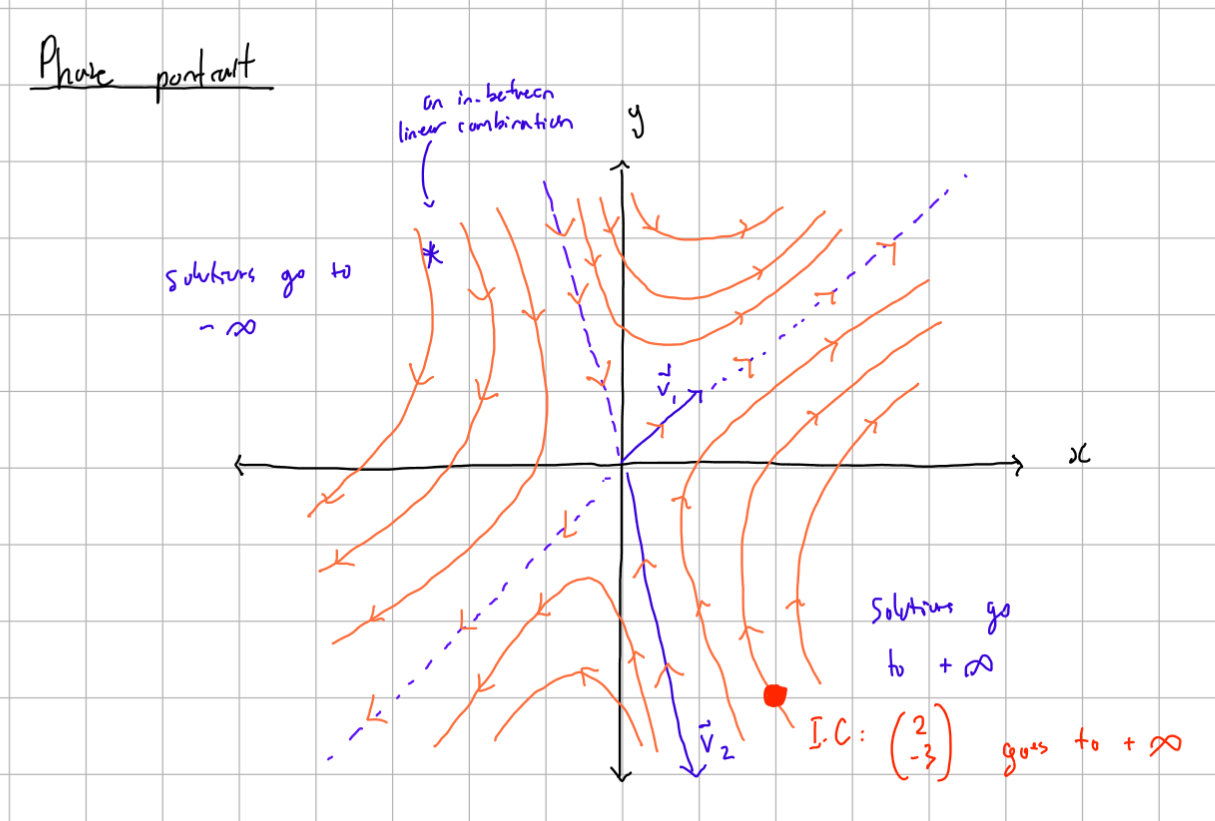
\includegraphics[width=0.9\textwidth]{images/linear_systems/phase_portrait_example1.png}
\end{center}

Note that the characteristic polynomial $\lambda^2 + \lambda -6 = p(\lambda)$ is exactly the same as the one-dimensional 2nd order system:
\begin{align*}
\ddot{x} = \frac{d}{dt} \dot{x} &= \frac{d}{dt} (x + y) \\
&= \dot{x} + \dot{y} \\
&= \dot{x} + 4x - 2y \\
&= \dot{x} + 4x - 2(\dot{x} - x) \\
&= -\dot{x} + 6x \\
\end{align*}

Then we have that $\ddot{x} + \dot{x} - 6x = 0$ has the same characteristic polynomial as the system of ODEs, and hence the same eigenvalues. This is a general result: the characteristic polynomial of a system of ODEs is the same as the characteristic polynomial of the corresponding higher-order ODE.


\section{Harmonic oscillators (complex eigenvalues)}
Consider the second-order ODE given by:
\begin{equation*}
\ddot{x} + \omega^2 x = 0
\end{equation*}

By using a change of variables $y = \dot{x}$, we can rewrite this as a system of ODEs:
\begin{equation*}
\begin{cases}
\dot{x} = y \\
\dot{y} = -\omega^2 x
\end{cases}
\end{equation*}

This system of ODEs can be represented in matrix form as:
\begin{equation*}
\begin{bmatrix}
\dot{x} \\
\dot{y}
\end{bmatrix} =
\begin{bmatrix}
0 & 1 \\
-\omega^2 & 0
\end{bmatrix}
\begin{bmatrix}
x \\
y
\end{bmatrix}
\end{equation*}

The characteristic polynomial of the matrix is given by:
\begin{align*}
\det \begin{bmatrix}
-\lambda & 1 \\
-\omega^2 & -\lambda
\end{bmatrix} &=
\lambda^2 + \omega^2 = 0
\end{align*}

This gives us the eigenvalues $\lambda = \pm i \omega$. We find that the eigenvectors are: 
\begin{equation*}
v_1 = \begin{bmatrix}
1 \\
i \omega
\end{bmatrix}, \quad v_2 = \begin{bmatrix}
1 \\
- i \omega
\end{bmatrix}
\end{equation*}

Then, we can write the general solution to the system of ODEs as:
\begin{equation*}
u(t) = c_1 e^{i \omega t} v_1 + c_2 e^{- i \omega t} v_2
\end{equation*}

We have a real solution, so the coefficients $c_1$ and $c_2$ must be complex. Using initial conditions $u(0) = \begin{bmatrix} 1 \\ 0 \end{bmatrix}$, we solve:
\begin{align*}
\begin{bmatrix}
1 \\
0
\end{bmatrix} &=
c_1 \begin{bmatrix}
1 \\
i \omega
\end{bmatrix} +
c_2 \begin{bmatrix}
1 \\
- i \omega
\end{bmatrix} \\
&=
\begin{bmatrix}
-i (c_1 - c_2) \\
\omega (c_1 + c_2)
\end{bmatrix}
\end{align*}

Then from $c_1 = -c_2$, we get $1 = -i (2c_2)$, so $c_2 = \frac{i}{2}$ and $c_1 = -\frac{i}{2}$. Thus, the solution to the system of ODEs is given by:
\begin{equation*}
u(t) = \frac{i}{2} e^{- i \omega t} v_2 - \frac{i}{2} e^{i \omega t} v_1
\end{equation*}

Using Euler's formula, we can rewrite this as:
\begin{equation*}
u(t) = \begin{bmatrix}
\cos(\omega t) \\
- \omega \sin(\omega t)
\end{bmatrix}
\end{equation*}

Now, plotting the phase portait of this system, we get cycles around the origin.
\begin{center}
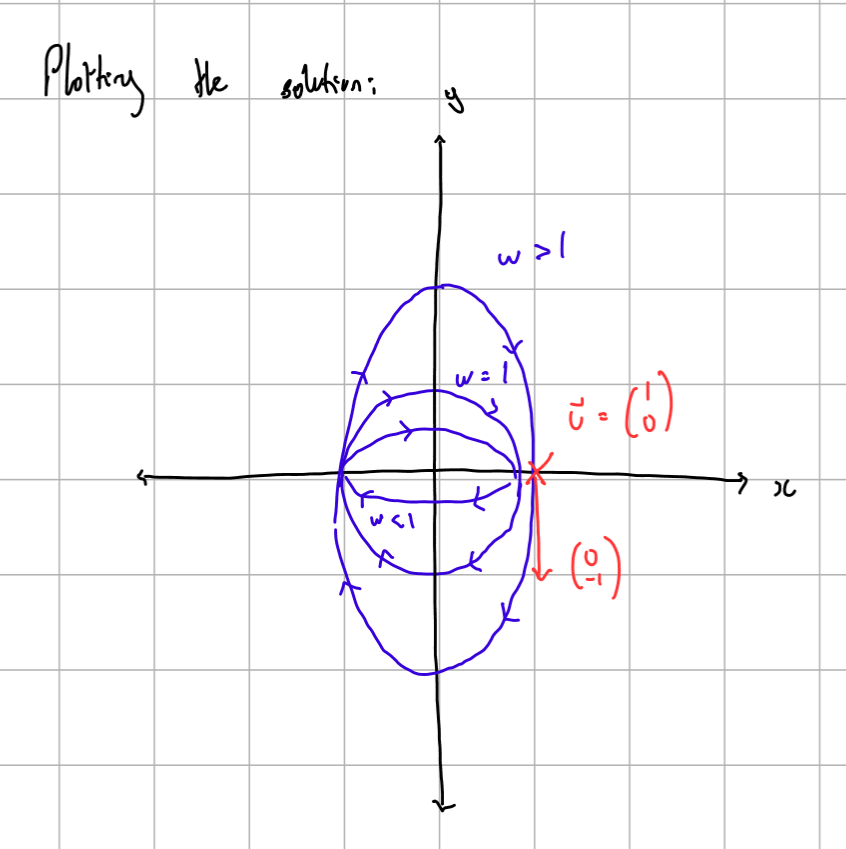
\includegraphics[width=0.9\textwidth]{images/linear_systems/phase_portrait_example2.png}
\end{center}

\ex{Love affair}{
    Consider two functions:
    \begin{equation*}
\begin{cases}
    R(t) = \text{Romeo's love for Juliet at time } t \\
    J(t) = \text{Juliet's love for Romeo at time } t
\end{cases}
    \end{equation*}

    We first consider when the love that Romeo has for Juliet depends only on Juliet's love for Romeo, and vice versa. Let $a, b > 0$, then:
\begin{equation*}
\begin{cases}
    \dot{R} = a J \\
    \dot{J} = -b R
\end{cases}
\end{equation*}
This system describes a situation where Romeo loves Juliet the more she loves him, but Juliet loves Romeo the less he loves her. We see that this is equivalent to the harmonic oscillator system above (with different coefficients), so we would observe cycling behaviour.

\begin{center}
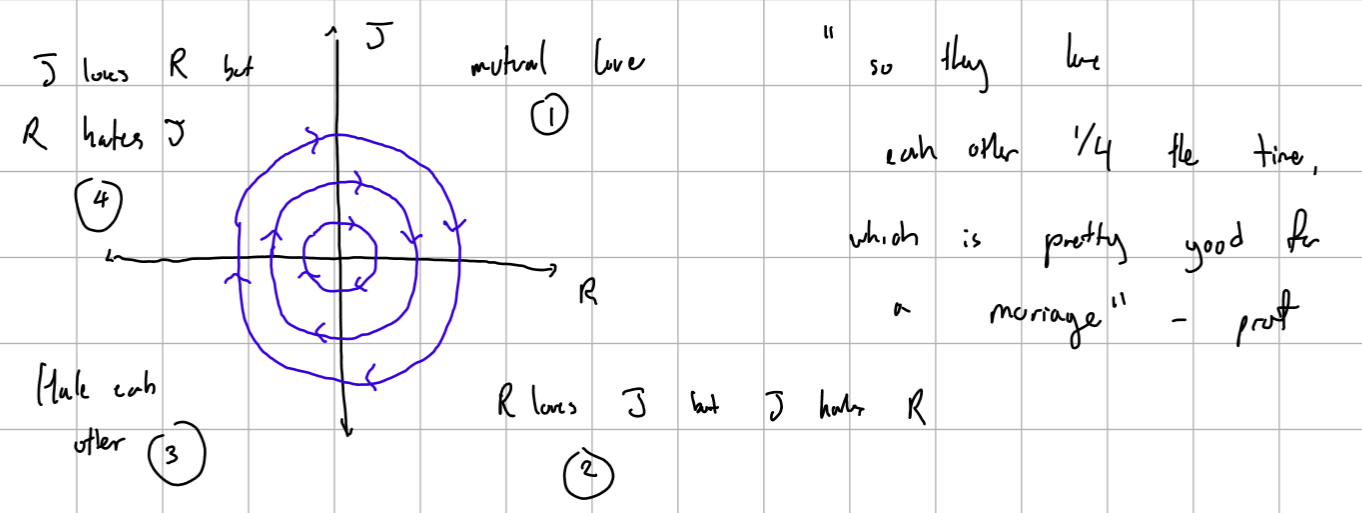
\includegraphics[width=0.6\textwidth]{images/linear_systems/love_affair_example1.png}
\end{center}

Now, we consider the general case:
\begin{equation*}
\begin{cases}
    \dot{R} = a R + b J \\
    \dot{J} = c R + d J
\end{cases}
\end{equation*}

The choice of sign for each coefficient signals the romantic style.

Consider a case where $a < 0$, $b > 0$, and we have:
\begin{equation*}
\begin{cases}
    \dot{R} = a R + b J \\
    \dot{J} = b R + a J
\end{cases}
\end{equation*}

Then the matrix of this system is given by:
\begin{equation*}
A = \begin{bmatrix}
a & b \\
b & a
\end{bmatrix}
\end{equation*}

It should be easy to see that the eigenvalues of this matrix are given by $\lambda_1 = a + b$ and $\lambda_2 = a - b$. Also, the eigenvectors are:
\begin{equation*}
v_1 = \begin{bmatrix}
1 \\
1
\end{bmatrix}, \quad v_2 = \begin{bmatrix}
1 \\
-1
\end{bmatrix}
\end{equation*}

We can also compute the determinant:
\begin{equation*}
\det(A) = a^2 - b^2
\end{equation*}

Then depending on the value of $a$ and $b$, we can have different behaviours:
\begin{itemize}
\item If $a^2 > b^2$, then the eigenvalues are real and negative, and the system is a stable node. The love affair will eventually die out. \\
\item If $a^2 < b^2$, then the eigenvalues are real and of opposite signs, and the system is a saddle. The love affair will be unstable, with one person loving the other more and more while the other person loves them less and less.
\end{itemize}

\begin{center}
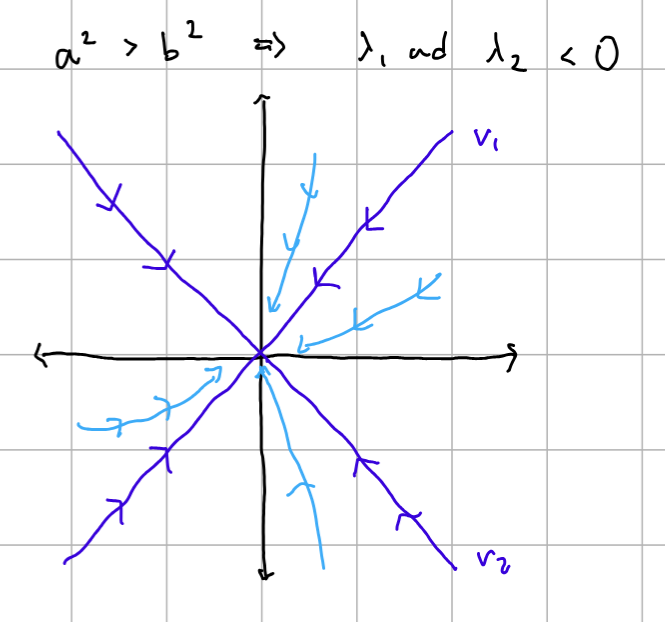
\includegraphics[width=0.5\textwidth]{images/linear_systems/love_affair_example2.png}
\end{center}

\begin{center}
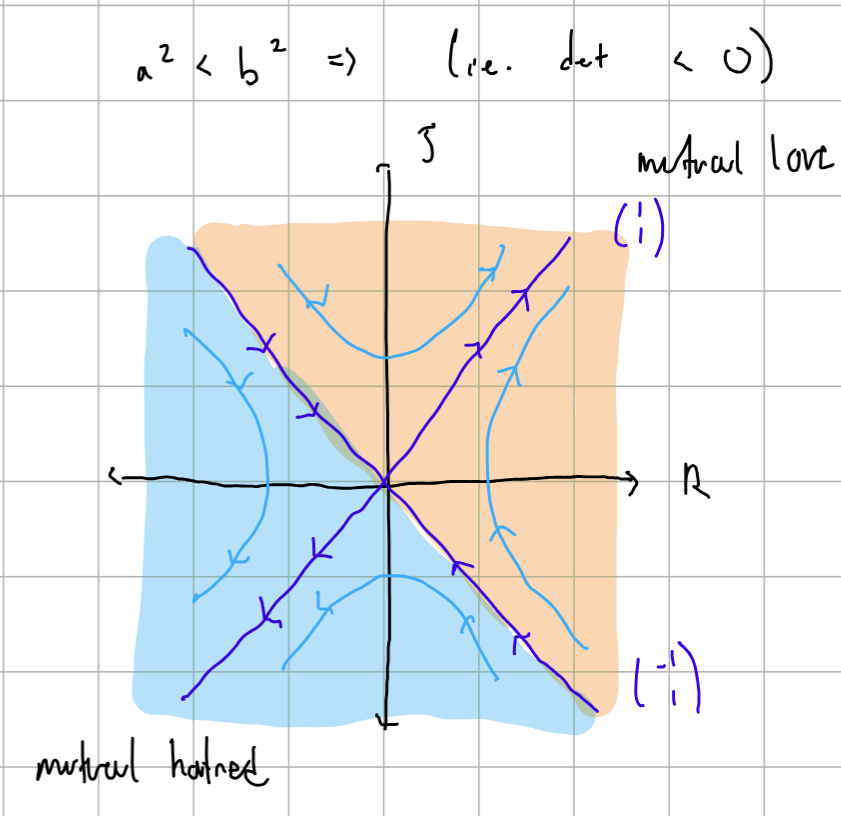
\includegraphics[width=0.5\textwidth]{images/linear_systems/love_affair_example3.png}
\end{center}
}

\section{Repeated eigenvalues}

Given the system $\dot{u} = Au$ (for a 2-dimensional system), if $A$ has a repeated eigenvalue, then:
\begin{itemize}
\item Then only one eigenvector  $v_1$ exists. 
\item There is only one fundamental solution given by: $u_1(t) = e^{\lambda t} v_1$ where $v_1$ is the eigenvector. 
\end{itemize}

We need another solution which is linearly independent from $v_1$.

\begin{mdframed}
\subsection{Finding a second solution when there is a repeated eigenvalue}
Let $v_1$ be the eigenvector corresponding to the repeated eigenvalue $\lambda$. We can find a second solution of the form:
\begin{equation*}
u_2(t) = e^{\lambda t} (t v_1 + w)
\end{equation*}
where $w$ is a vector that we need to determine.

Plug $u_2 (t)$ into $\dot{u} = Au$:
\begin{align*}
\dot{u}_2(t) &= A u_2(t) \\
e^{\lambda t} (v_1 + t \lambda v_1 + \lambda w) &= e^{\lambda t} (t A v_1 + A w) \\
v_1 + t \lambda v_1 + \lambda w &= t \lambda v_1 + A w \quad \text{ using } Av_1 = \lambda v_1\\ 
v_1 + \lambda w &= A w
\end{align*}


Rearranging this, we get:
\begin{equation*}
(A - \lambda I) w = v_1
\end{equation*}
Since $v_1$ is an eigenvector corresponding to $\lambda$, we know that $(A - \lambda I) v_1 = 0$. Thus, the matrix $A - \lambda I$ is singular, and we can find a solution for $w$ using methods such as Gaussian elimination or by finding the null space of $A - \lambda I$.
\end{mdframed}

The general solution to the system of ODEs in this case is given by:
\begin{equation*}
\boxed{
u(t) = c_1 e^{\lambda t} v_1 + c_2 e^{\lambda t} (t v_1 + w)
}
\end{equation*}

\ex{Example of repeated eigenvalues}{
    Consider the system of ODEs given by:
\begin{equation*}
\begin{cases}
\dot{x} = 2x + y \\
\dot{y} = -4x - 2y
\end{cases}
\end{equation*}
We can write this system in matrix form as:
\begin{equation*}
\begin{bmatrix}
\dot{x} \\
\dot{y}
\end{bmatrix} =
\begin{bmatrix}
2 & 1 \\
-4 & -2
\end{bmatrix}
\begin{bmatrix}
x \\
y
\end{bmatrix}
\end{equation*}

We will find that $\lambda = 0$ is a repeated eigenvalue, and that $u_1(t) = \begin{bmatrix}
1 \\
-2
\end{bmatrix}$ is the corresponding eigenvector.

Then, we can find $w$ by solving:
\begin{equation*}
\begin{bmatrix}
2 & 1 \\
-4 & -2
\end{bmatrix}
\begin{bmatrix}
w_1 \\
w_2
\end{bmatrix} =
\begin{bmatrix}
1 \\
-2
\end{bmatrix}
\end{equation*}

We can row-reduce this matrix to find a solution for $w$:
\begin{equation*}
\begin{bmatrix}
2 & 1 & 1 \\
-4 & -2 & -2
\end{bmatrix} \to
\begin{bmatrix}
1 & \frac{1}{2} & \frac{1}{2} \\
0 & 0 & 0
\end{bmatrix}
\end{equation*}

This gives us: $2a + b = 1$. We could choose $a = 0$ and $b = 1$, then:
\begin{equation*}
w = \begin{bmatrix}
0 \\
1
\end{bmatrix}
\end{equation*}

Thus, the general solution to the system of ODEs is given by:
\begin{equation*}
u(t) = c_1 
\begin{bmatrix}
1 \\
-2 
\end{bmatrix} +
c_2 
\left(
t 
\begin{bmatrix}
1 \\ 
-2
\end{bmatrix}
+ 
\begin{bmatrix}
0 \\
1
\end{bmatrix}
\right)
\end{equation*}
}



